\documentclass[12pt]{iopart}
\pdfoutput=1
\usepackage{iopams}
\usepackage{amssymb, epsfig}
%\usepackage{amsmath, amssymb,epsfig}
\usepackage{latexsym}

%\usepackage[hypertex,hyperindex]{hyperref}
%\usepackage{showkeys}
\usepackage{graphicx}
\usepackage{color}

\newcommand{\pf}{\mbox{pf}}
\newcommand{\vep}{\varepsilon}

\begin{document}

\bibliographystyle{plain}
\def\debproof{\noindent {\bf Proof.} }
\def\finproof{\hfill {\small $\Box$} \\}
%\renewcommand{\theequation}{\arabic{section}.\arabic{equation}}
%\tableofcontents
\makeatletter % `@' now normal "letter"
\@addtoreset{equation}{section}
\makeatother  % `@' is restored as "non-letter"
\renewcommand\theequation{{\thesection}.{\arabic{equation}}}

\title[]{Scattering Coefficient and Kirchhoff Approximation}
\author{ }
\address{}



\maketitle

\newcommand{\eps}{\varepsilon}
\newcommand{\RR}{\mathcal{R}}
\newtheorem{lem}{Lemma}[section]
\newtheorem{prop}{Proposition}[section]
\newtheorem{cor}{Corollary}[section]
\newtheorem{thm}{Theorem}[section]
\newtheorem{rem}{Remark}[section]
\newtheorem{alg}{Algorithm}[section]
\newtheorem{assum}{Assumption}[section]
\newtheorem{definition}{Definition}[section]


\newcounter{RomanNumber}
\newcommand{\MyRoman}[1]{\rm\setcounter{RomanNumber}{#1}\Roman{RomanNumber}}

\newcommand{\bL}{\mathbf{L}}
\newcommand{\bH}{\mathbf{H}}
\newcommand{\bW}{\mathbf{W}}
\newcommand{\bP}{\mathbf{P}}
\newcommand{\bQ}{\mathbf{Q}}
\newcommand{\bp}{\mathbf{p}}
\newcommand{\bq}{\mathbf{q}}
\newcommand{\uL}{u_{_{\rm L}}}
\newcommand{\vL}{v_{_{\rm L}}}
\newcommand{\tuL}{\tilde u_{_{\rm L}}}
\newcommand{\tvL}{\tilde v_{_{\rm L}}}
\newcommand{\fL}{f_{_{\rm L}}}
\newcommand{\gL}{g_{_{\rm L}}}
\newcommand{\bpL}{\bp_{_{\rm L}}}
\newcommand{\bqL}{\bq_{_{\rm L}}}
\newcommand{\tbpL}{\tilde{\bp}_{_{\rm L}}}
\newcommand{\tbqL}{\tilde{\bq}_{_{\rm L}}}
\newcommand{\tbpLf}{\tilde{\bp}_{_{\rm L,1}}}
\newcommand{\tbpLs}{\tilde{\bp}_{_{\rm L,2}}}
\newcommand{\tbqLf}{\tilde{\bq}_{_{\rm L,1}}}
\newcommand{\tbqLs}{\tilde{\bq}_{_{\rm L,2}}}
\newcommand{\bn}{\nu}
\newcommand{\bv}{\mathbf{v}}
\newcommand{\om}{\omega}
\newcommand{\pa}{\partial}
\newcommand{\la}{\langle}
\newcommand{\ra}{\rangle}
\newcommand{\lla}{\la{\hskip -2pt}\la}
\newcommand{\rra}{\ra{\hskip -2pt}\ra}
\newcommand{\jj}{\|{\hskip -0.8pt} |}
\newcommand{\al}{\alpha}
\newcommand{\ze}{\zeta}
\newcommand{\si}{\sigma}
\newcommand{\ep}{\varepsilon}
\newcommand{\na}{\nabla}
\newcommand{\vp}{\varphi}
\newcommand{\ga}{\gamma}
\newcommand{\Ga}{\Gamma}
\newcommand{\Om}{\Omega}
\newcommand{\de}{\delta}
\newcommand{\Th}{\Theta}
\newcommand{\De}{\Delta}
\newcommand{\Lam}{\Lambda}
\newcommand{\lam}{\lambda}
\newcommand{\tri}{\triangle}
\newcommand{\lj}{[{\hskip -2pt} [}
\newcommand{\rj}{]{\hskip -2pt} ]}
\newcommand{\bks}{\backslash}
%\newcommand{\diag}{\mathrm{diag}}
\newcommand{\diam}{\mathrm{diam}}
\newcommand{\osc}{\mathrm{osc}}
\newcommand{\meas}{\mathrm{meas}}
\newcommand{\dist}{\mathrm{dist}}

\newcommand{\mL}{\mathscr{L}}
\newcommand{\cT}{{\cal T}}
\newcommand{\cM}{{\cal M}}
\newcommand{\cE}{{\cal E}}
\newcommand{\cL}{{\cal L}}
\newcommand{\cF}{{\cal F}}
\newcommand{\cB}{{\cal B}}
\newcommand{\PML}{{\rm PML}}
\newcommand{\FEM}{{\rm FEM}}
\newcommand{\rd}{\,\mathrm{d}}

\renewcommand{\i}{\mathbf{i}}
\renewcommand{\v}{\mathbf{v}}
\renewcommand{\u}{\mathbf{u}}
\renewcommand{\r}{\mathbf{r}}
\newcommand{\gR}{{\mathbb{R}}}
\newcommand{\Z}{{\mathbb{Z}}}
\newcommand{\C}{{\mathbb{C}}}
\newcommand{\I}{{\mathbb{I}}}
\renewcommand{\Re}{\mathrm{Re}\,}
\renewcommand{\Im}{\mathrm{Im}\,}
\renewcommand{\div}{\mathrm{div}}
\newcommand{\curl}{\mathrm{curl}}
\newcommand{\Curl}{\mathbf{curl}}
\newcommand{\pv}{\mathrm{p.v.}}

\newcommand{\Np}{\mathbb{N}_p}
\newcommand{\Ns}{\mathbb{N}_s}
\newcommand{\Tp}{\mathbb{T}_p}
\newcommand{\Ts}{\mathbb{T}_s}
\newcommand{\Na}{\mathbb{N}_\alpha}
\newcommand{\Nb}{\mathbb{N}_\beta}
\newcommand{\Ta}{\mathbb{T}_\alpha}
\newcommand{\Tb}{\mathbb{T}_\beta}
\newcommand{\GG}{\mathcal{G}}

\newcommand{\N}{\mathbb{N}}
\newcommand{\D}{\mathbb{D}}
\newcommand{\T}{\mathbb{T}}
\newcommand{\A}{\mathbb{A}}
\newcommand{\B}{\mathbb{B}}
\newcommand{\G}{\mathbb{G}}
\newcommand{\F}{\mathbb{F}}
\newcommand{\R}{\mathbb{R}}
\newcommand{\W}{\mathbb{W}}
\newcommand{\V}{\mathbb{V}}
\newcommand{\U}{\mathbb{U}}
\newcommand{\J}{\mathbb{J}}
\newcommand{\Zg}{\mathbb{Z}}
\newcommand{\Gtheta}{\mathbb{\Theta}}
\newcommand{\Gphi}{\mathbb{\Phi}}

%%%%%%%%%%%%%%%%%%%%%%%%%%%%%%%%%%%%%%%%%%%%%%%%%%%%%%%%%%%%%%%%%%%%
\newcommand{\be}{\begin{eqnarray}}
\newcommand{\ee}{\end{eqnarray}}
\newcommand{\ben}{\begin{eqnarray*}}
	\newcommand{\een}{\end{eqnarray*}}
\newcommand{\nn}{\nonumber}

\section{Introdution}

we introduce the concept of the scattering coefficient for incident plane waves.

\begin{definition} \label{def:4.1} For any unit vector $\eta\in\R^2$, let $v^i=e^{\i kx\cdot\eta}$ be the incident wave and $v^s=v^s(x,\eta)$ be the
	radiation solution of the Helmholtz equation:
	\ben
	\Delta v^s+k^2v^s=0\ \ \mbox{\rm in }\R^2\backslash\bar D,\ \ v^s=-e^{\i kx\cdot\eta}\ \ \mbox{\rm on }\Ga_D.
	\een
	The scattering coefficient $R(x,\eta)$ for $x\in\Ga_D$ is defined by the relation
	\ben
	\frac{\pa(v^s+v^i)}{\pa\nu}=\i kR(x,\eta)e^{\i kx\cdot\eta}\ \ \ \ \mbox{\rm on }\Ga_D.
	\een
\end{definition}
In the case of Kirchhoff high frequency approximation and the mathematical justification for strictly convex obstacles, the scattering coefficient can be approximated by
\ben
R(x,\eta)=\left\{\begin{array}{ll}
	2\nu(x)\cdot\eta & \mbox{If }x\in\pa D_\eta^-:=\{x\in\Ga_D:\nu(x)\cdot\eta<0\},\\
	0 & \mbox{If }x\in\pa D_\eta^+:=\{x\in\Ga_D:\nu(x)\cdot\eta>0\}.\\
\end{array}\right.
\een
Here $\pa D_\eta^-$ and $\pa D^+_\eta$ are respectively the illuminating and shadow region for the incident wave $e^{\i kx\cdot\eta}$. 

\section{Numerical Tests}
\begin{figure}
	\centering
	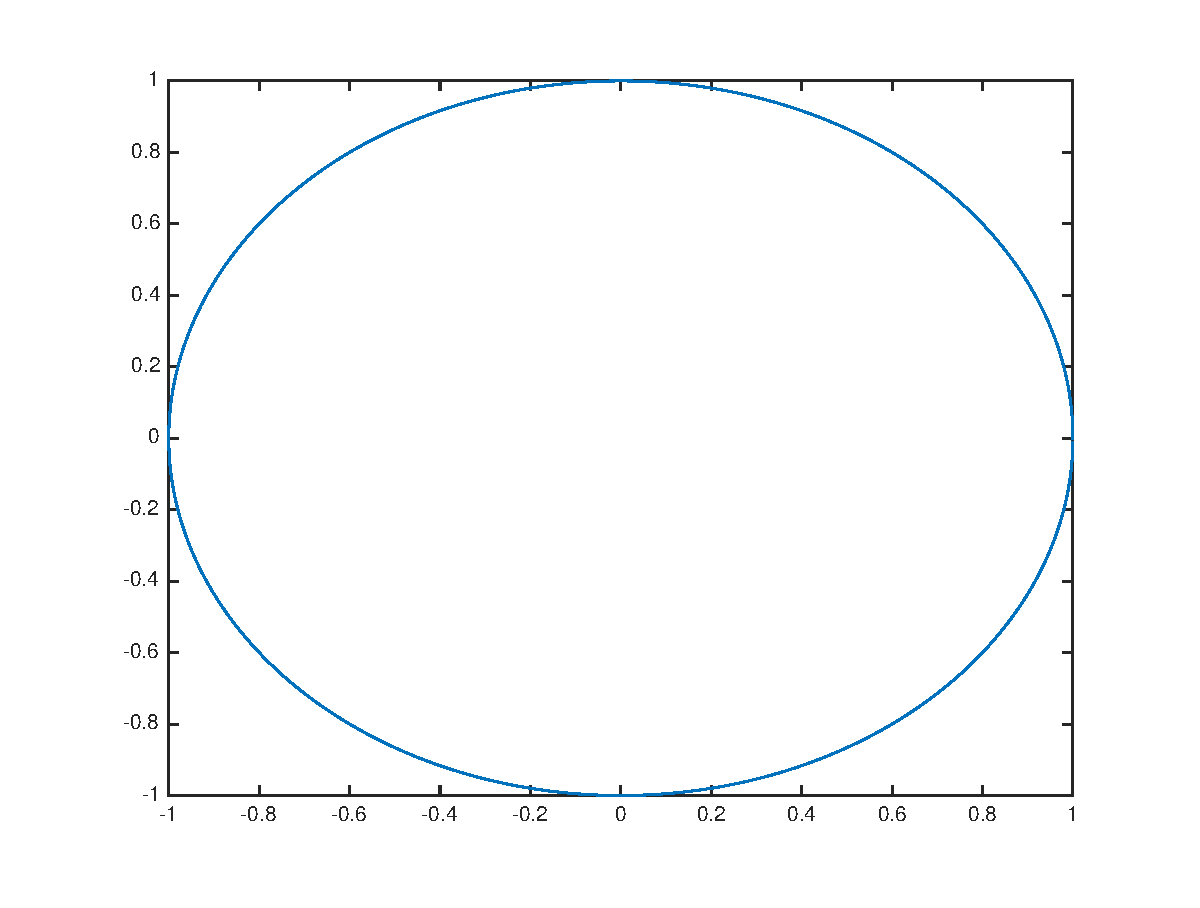
\includegraphics[width=0.24\textwidth]{./figure_sc/circle.eps}
	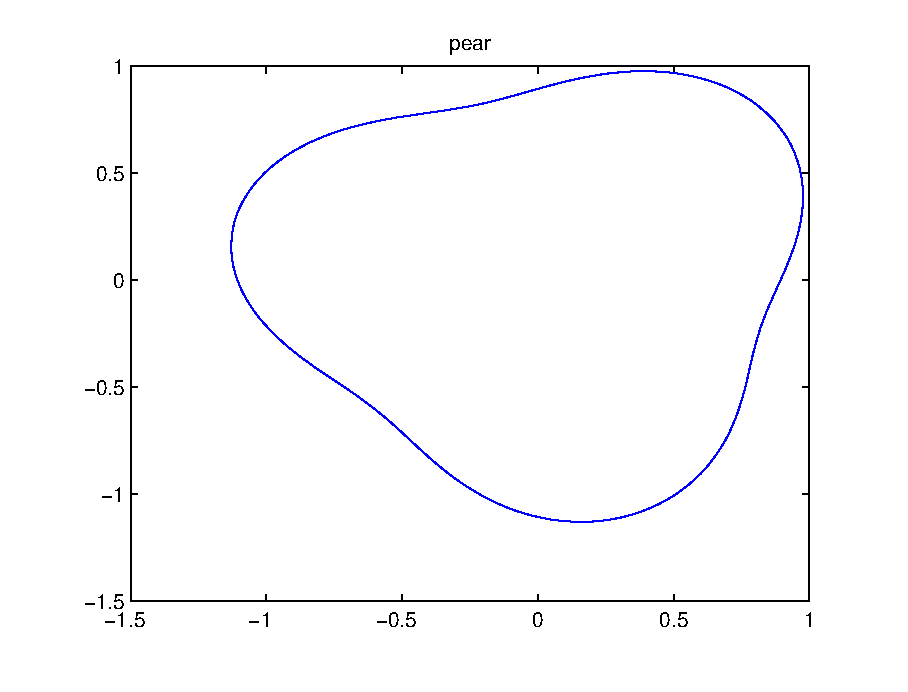
\includegraphics[width=0.24\textwidth]{./figure_sc/pear.eps}
	\includegraphics[width=0.24\textwidth]{./figure_sc/rectangle.eps}
	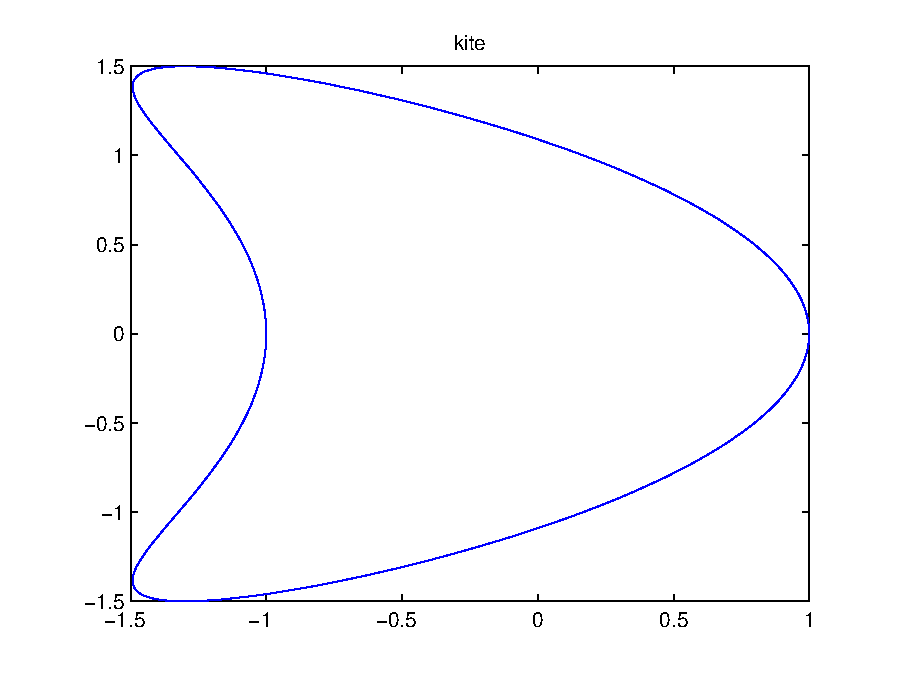
\includegraphics[width=0.24\textwidth]{./figure_sc/kite.eps}
	\caption{}\label{shape}
\end{figure}
\begin{figure}
	\centering
	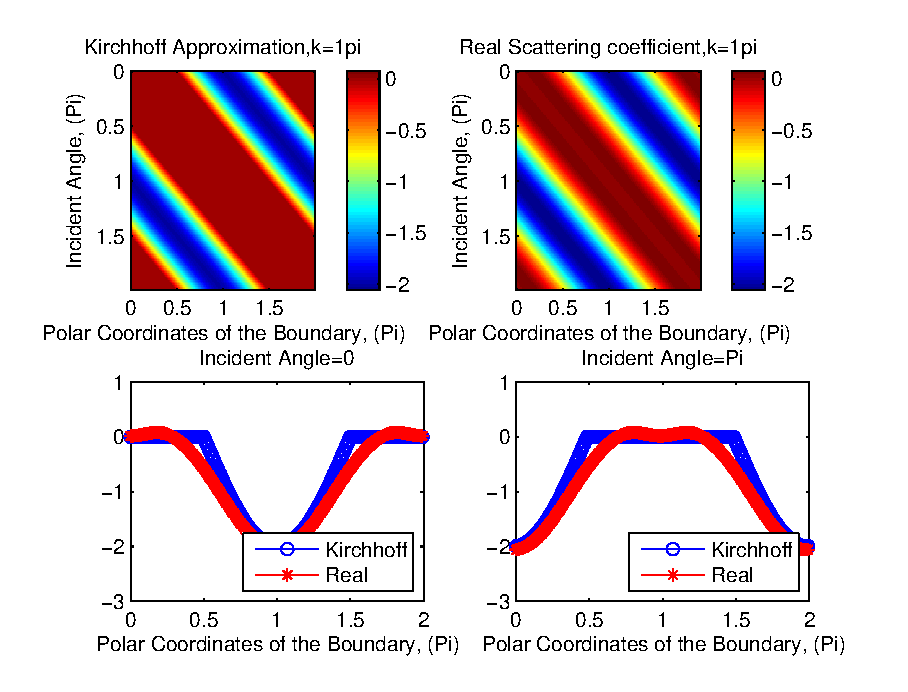
\includegraphics[width=0.6\textwidth]{./figure_sc/scattering_coefficient_circle_1.eps}
	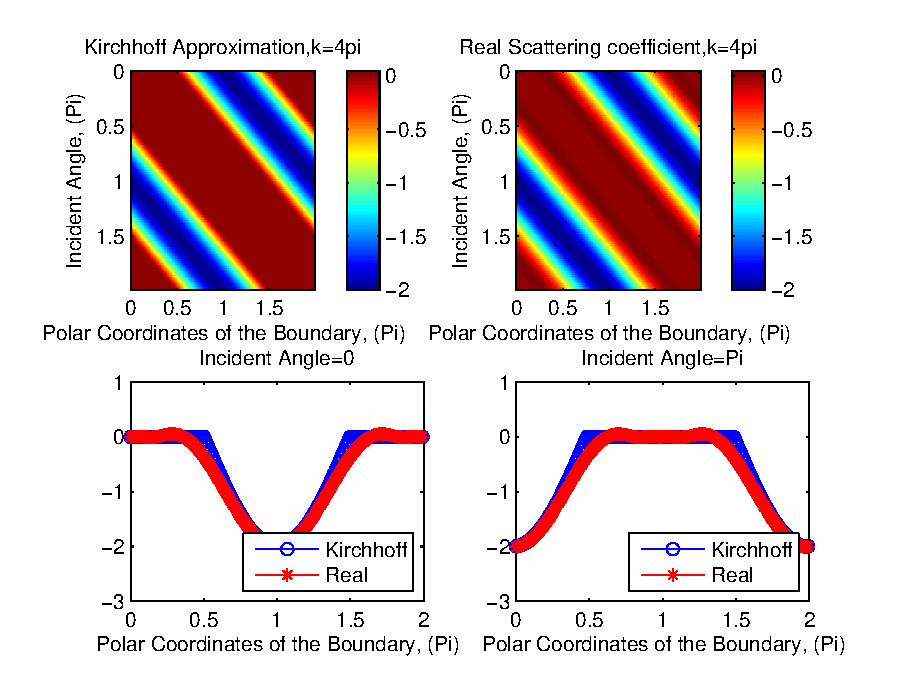
\includegraphics[width=0.6\textwidth]{./figure_sc/scattering_coefficient_circle_4.eps}
	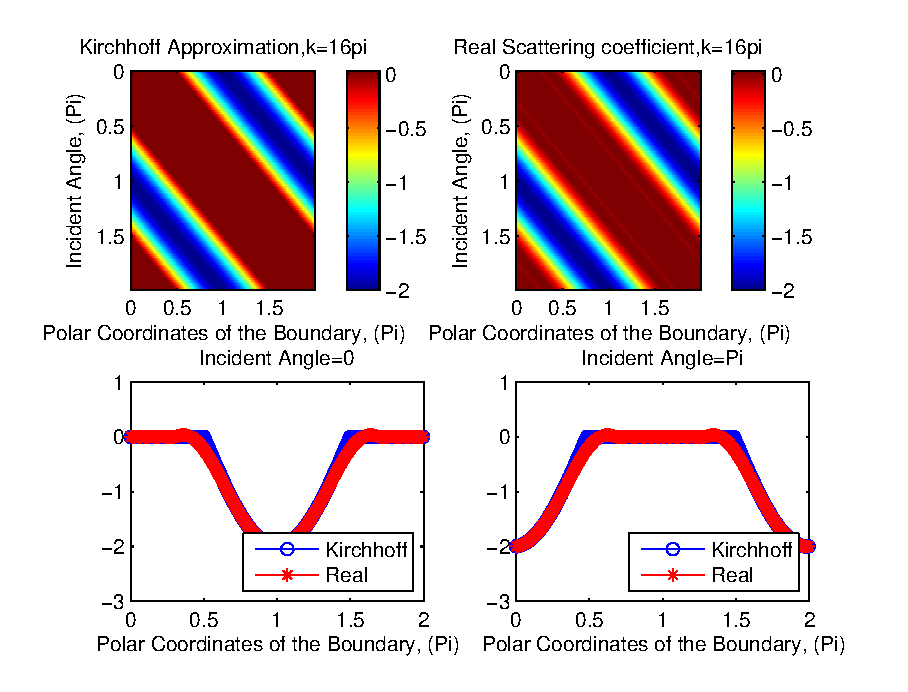
\includegraphics[width=0.6\textwidth]{./figure_sc/scattering_coefficient_circle_16.eps}
	\caption{}\label{circle}
\end{figure}
\begin{figure}
	\centering
	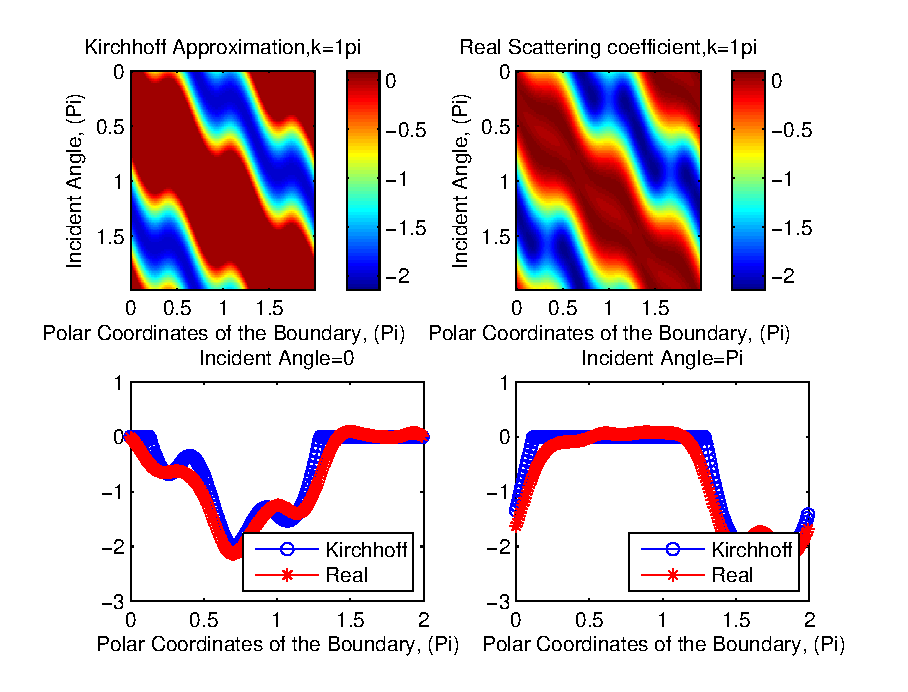
\includegraphics[width=0.6\textwidth]{./figure_sc/scattering_coefficient_pear_1.eps}
	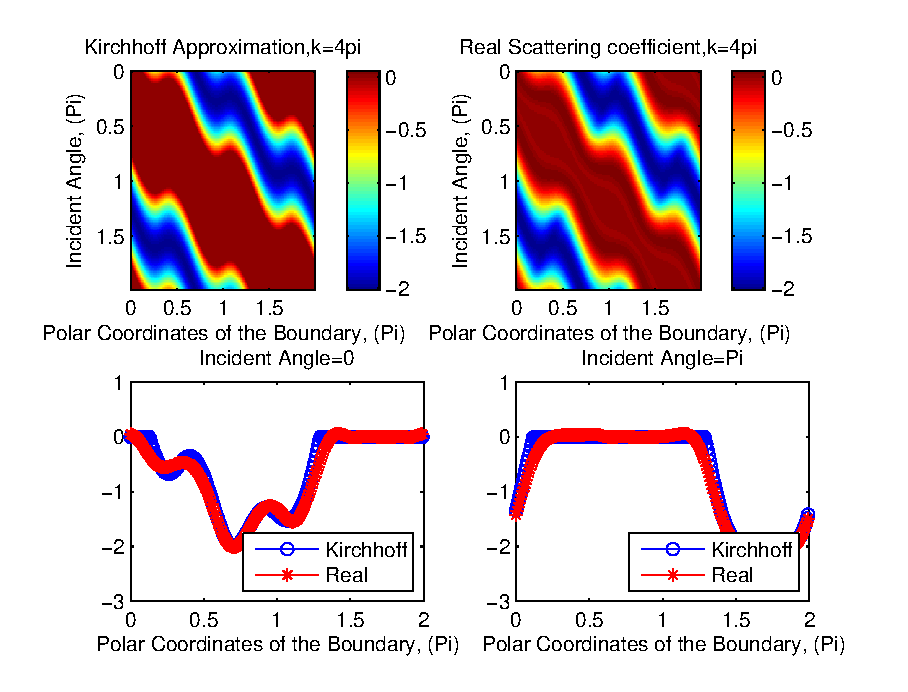
\includegraphics[width=0.6\textwidth]{./figure_sc/scattering_coefficient_pear_4.eps}
	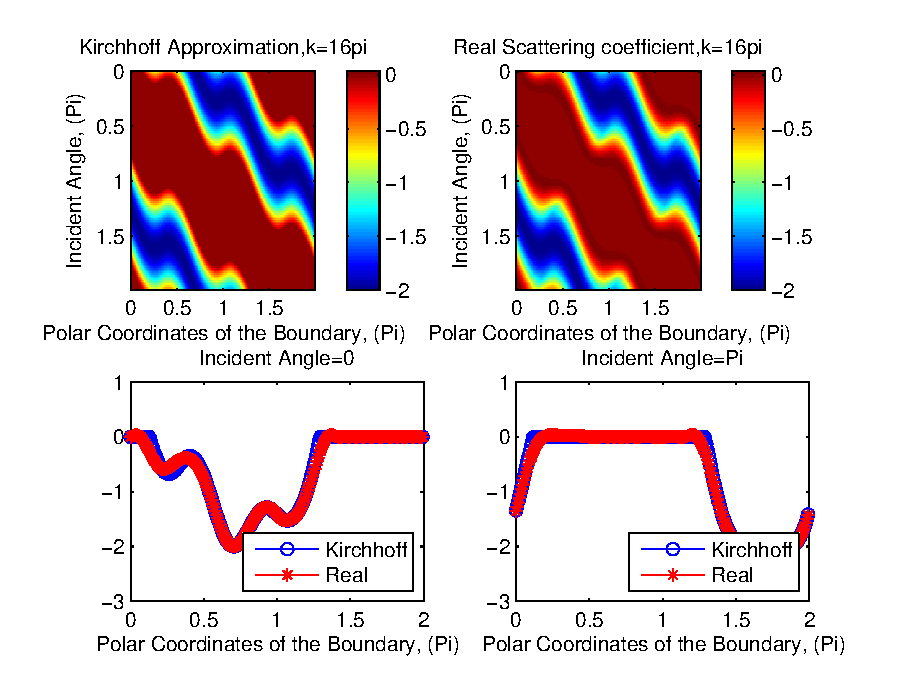
\includegraphics[width=0.6\textwidth]{./figure_sc/scattering_coefficient_pear_16.eps}
	\caption{}\label{pear}
\end{figure}
\begin{figure}
	\centering
	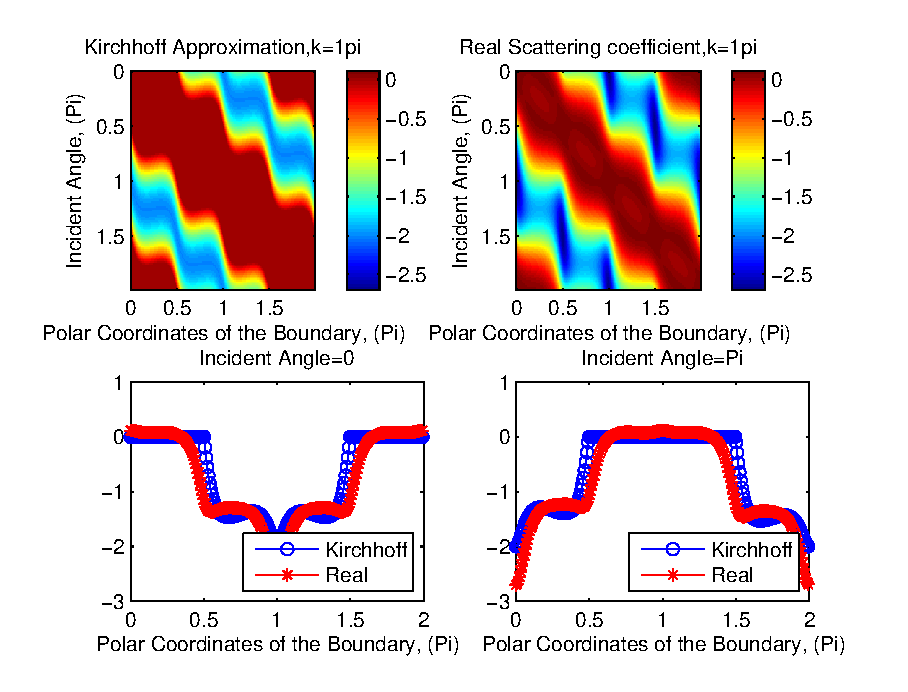
\includegraphics[width=0.6\textwidth]{./figure_sc/scattering_coefficient_rctangle_1.eps}
	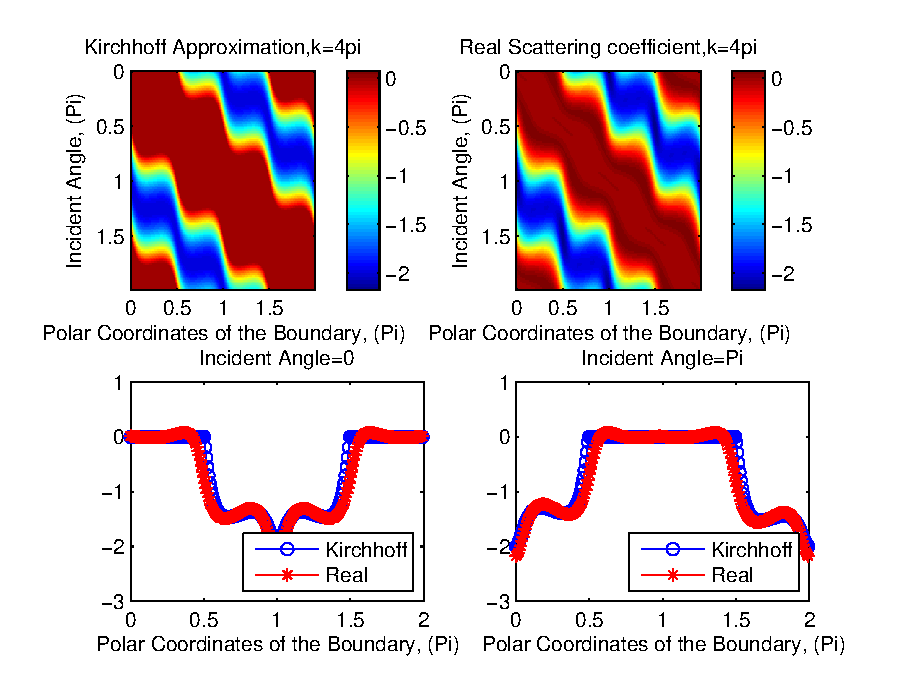
\includegraphics[width=0.6\textwidth]{./figure_sc/scattering_coefficient_rctangle_4.eps}
	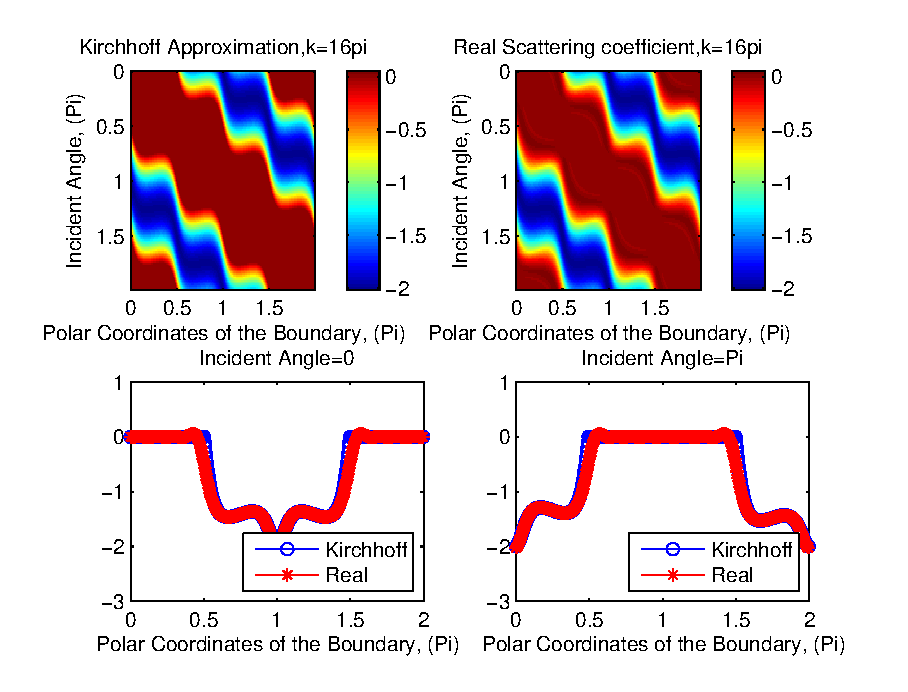
\includegraphics[width=0.6\textwidth]{./figure_sc/scattering_coefficient_rctangle_16.eps}
	\caption{}\label{rectangle}
\end{figure}
\begin{figure}
	\centering
	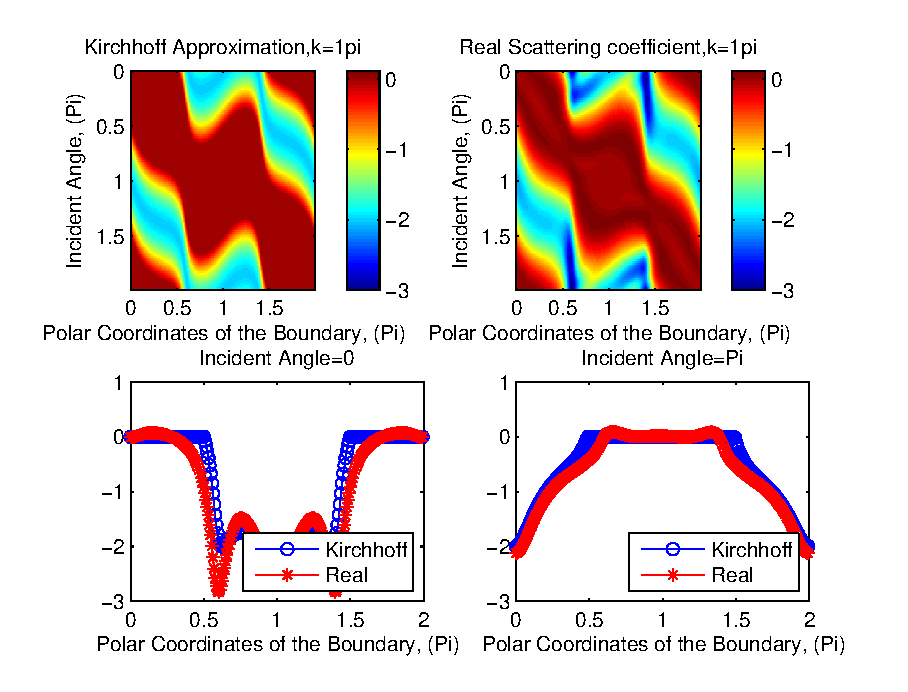
\includegraphics[width=0.6\textwidth]{./figure_sc/scattering_coefficient_kite_1.eps}
	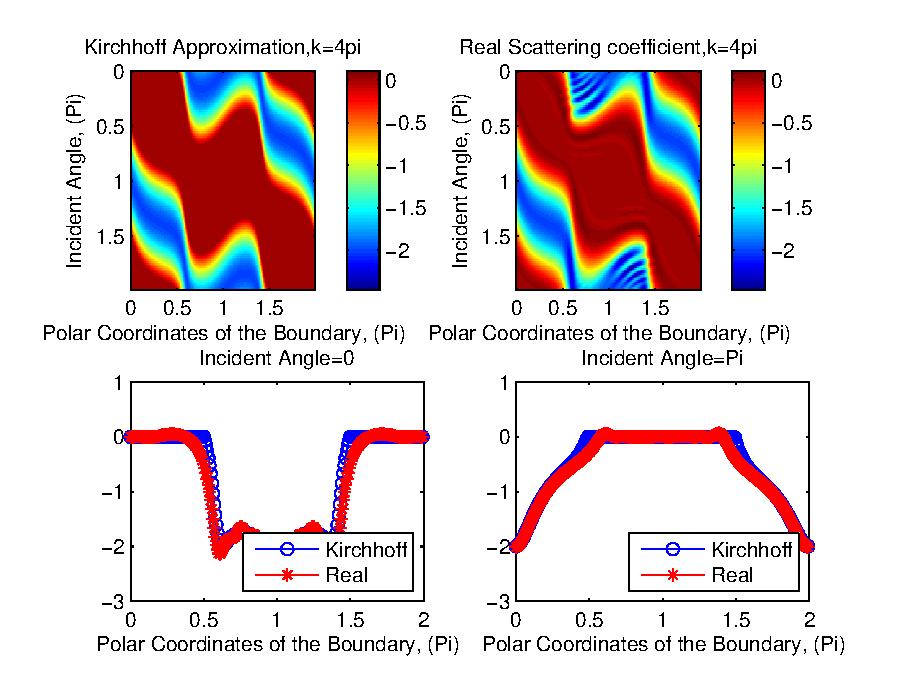
\includegraphics[width=0.6\textwidth]{./figure_sc/scattering_coefficient_kite_4.eps}
	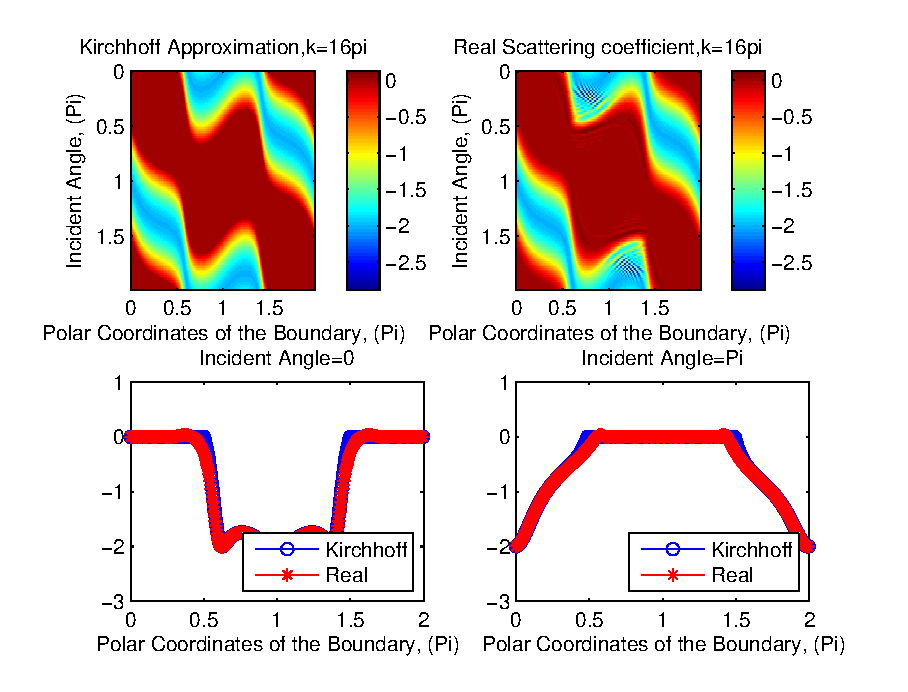
\includegraphics[width=0.6\textwidth]{./figure_sc/scattering_coefficient_kite_16.eps}
	\caption{}\label{kite}
\end{figure}
\end{document}
